% Provenance (never printed): see sources/outline_sources.md (Year 3:
% planetary atmospheres, escape, the runaway greenhouse, Mars, Titan,
% habitability).
% Brief: sources/book5/BRIEFS.md, ch. 27. Curves from figdata/bachelor-3/
% jeans_escape.py (escape parameter and escaping fraction at the exobases
% of Venus, the Earth, Mars and Titan), runaway_greenhouse.py (an
% illustrative grey model of a moist atmosphere: OLR against surface
% temperature) and habitability.py (the habitable-zone fits of Kopparapu et
% al. 2013; the phase boundaries of water and methane with the surface
% states of four bodies). Exercise and problem values in the Book 5 scratch
% calculator calc/ch27.py. Kepos and its star are invented.
\chapter{Planetary Atmospheres and Habitability}\label{ch:b3:planetary-atmospheres}

Venus and the Earth are near twins: almost the same size, similar mean
densities, neighbouring orbits. Yet Venus keeps \qty{92}{bar} of carbon
dioxide over a surface at \qty{737}{K}, and so little water that, spread
over its surface, it would make a layer about a centimetre deep. The mass
spectrometer of the Pioneer Venus probe, falling through its clouds,
measured the ratio of deuterium to hydrogen in that water: \num{0.016},
a hundred times the ratio in the Earth's oceans. Light hydrogen escapes to
space more easily than heavy deuterium; what is left of a large reservoir
that has lost most of its hydrogen is rich in deuterium. The ratio is the
trace of water that Venus once had, and lost. This chapter asks how a
planet holds on to its air and its water, and how it loses them.
% ledger: planet:Venus.diameter, planet:Earth.diameter, planet:Venus.density, planet:Earth.density, nasa:venus-atm, arney18:venus-water, donahue82:dh, kc98:standards

\begin{recall}
The scale height, the barometric formula, the Maxwell--Boltzmann
distribution, the escape velocity, the mean free path and the greenhouse
effect are in the physics books. The habitable zone of a star is in the
school books. The equilibrium temperature and the Bond albedo are in the
Year~1 volume, in its chapter on comparative planetology; the optical
depth, in its chapter on telescopes and photometry; the lapse rates, in
its chapter on the structure of the atmosphere and the ocean; the outgoing
longwave radiation (OLR) and the emission temperature, in its chapter on
radiation and heat transport. The moist adiabat is in the Year~2 volume,
in its chapter on atmospheric thermodynamics; the snow line, in its
chapter on planet formation; the long-term carbon cycle and the
silicate-weathering thermostat, in its chapter on climate over geological
time. \omterm{prop:b3:stable-isotopes:rayleigh-distillation}{Rayleigh distillation} is in this volume, in its chapter on stable
isotopes.
\end{recall}

\section{The structure of an atmosphere}\label{sec:b3:planetary-atmospheres:structure}

An isothermal atmosphere of molecular mass $m$ at temperature $T$ thins
with height as $p = p_0\,e^{-z/H}$, with the scale height $H = kT/mg$. At
the surface of the Earth $H$ is about \qty{8}{km}; at the surface of
Titan, where gravity is weak and the air cold, about \qty{20}{km}.

The temperature, though, is not uniform. Sunlight that reaches the ground
warms it; the air above, which absorbs and emits in the infrared, is
warmed from below. Radiation alone would make the lower atmosphere so
steep in temperature that it would overturn.

\begin{definition}[Radiative--convective equilibrium]\label{def:b3:planetary-atmospheres:rce}
A column of atmosphere is in \emph{radiative--convective
equilibrium}\index{radiative--convective equilibrium} when, at every
level, the net flux of radiation is balanced, except in a lower layer
where convection carries heat upwards and holds the temperature gradient
at the adiabatic one. The lower, convective layer is the troposphere; the
upper layer, in radiative equilibrium, the stratosphere; the tropopause
is the level where they meet.
\end{definition}

The simplest atmosphere in which this can be followed is \emph{grey}: it
is transparent to sunlight and absorbs every infrared wavelength alike,
with an optical depth $\tau$ counted downwards from the top.

\begin{proposition}[Grey radiative equilibrium]\label{prop:b3:planetary-atmospheres:grey}
In a grey atmosphere in radiative equilibrium that emits the flux $F$ to
space, the temperature at the optical depth $\tau$ obeys
\[
\sigma T^4(\tau) = \frac F2\,(1 + D\tau),
\]
where $D \approx 1.66$ accounts for the slant paths of the radiation.
The top of the atmosphere is at the \emph{skin temperature}
$T_\mathrm{skin} = 2^{-1/4}\,T_e$, where $T_e = (F/\sigma)^{1/4}$ is the
emission temperature.
\end{proposition}

The proposition is admitted; it follows from the two-stream equations for
the upward and downward fluxes. Where $\tau$ is large, near the ground,
the radiative temperature changes fast with $\tau$, and $\tau$ itself
grows quickly with depth because the absorbing gas is densest there: the
radiative profile is steeper than the adiabat, and convection takes over.
High up, $\tau$ is small and the temperature tends to the skin
temperature. The Earth emits about \qty{239}{W.m^{-2}} to space, an
emission temperature of \qty{255}{K} and a skin temperature of
\qty{214}{K}; the standard atmosphere sets its tropopause at \qty{11}{km}
and \qty{216.65}{K}. The grey model, crude as it is, places the cold top of
the troposphere about right.
% ledger: ipcc:budget-toa, ussa76:sea-level, ussa76:layers, const:sigma

\begin{omfigure}
\centering
\begin{tikzpicture}[x=1cm, y=0.8cm, font=\small]
% temperature profile (schematic)
\draw[->] (0,0) -- (6.8,0) node[below left, font=\scriptsize] {temperature};
\draw[->] (0,0) -- (0,8.4) node[above, font=\scriptsize] {height};
\draw[thick, omDef] (5.6,0) -- (4.2,2.0) -- (4.2,2.6) -- (4.7,3.6)
  -- (3.8,4.6) .. controls (4.3,5.6) and (5.9,6.0) .. (6.2,6.6) -- (6.25,8.2);
\draw[dashed, black!50] (0,2.0) -- (6.8,2.0) node[right, font=\scriptsize, black] {tropopause};
\draw[dashed, black!50] (0,4.6) -- (6.8,4.6) node[right, font=\scriptsize, black] {homopause};
\draw[thick, red!70!black] (0,6.6) -- (6.8,6.6) node[right, font=\scriptsize] {exobase};
\node[anchor=west, font=\scriptsize] at (0.15,0.9) {troposphere: convection};
\node[anchor=west, font=\scriptsize] at (0.15,0.5) {(adiabat)};
\node[anchor=west, font=\scriptsize] at (0.15,3.2) {stratosphere:};
\node[anchor=west, font=\scriptsize] at (0.15,2.8) {radiative equilibrium};
\node[anchor=west, font=\scriptsize] at (0.15,5.6) {thermosphere};
\node[anchor=west, font=\scriptsize] at (0.15,5.2) {(heated by EUV)};
\node[anchor=west, font=\scriptsize] at (0.15,7.6) {exosphere:};
\node[anchor=west, font=\scriptsize] at (0.15,7.2) {no collisions};
% exosphere trajectories
\begin{scope}[shift={(11.0,0)}]
\fill[black!8] (-2.3,0) rectangle (2.3,6.6);
\draw[red!70!black, thick] (-2.3,6.6) -- (2.3,6.6);
\node[font=\scriptsize] at (0,0.5) {collisions everywhere};
\node[font=\scriptsize, align=center] at (0,3.3) {gas mixed by\\turbulence below the\\homopause, separated\\by molecular diffusion\\above it};
\draw[->, thick, omDef] (-1.6,6.6) .. controls (-1.4,8.0) and (-0.9,8.0) .. (-0.7,6.6);
\node[font=\scriptsize, omDef] at (-1.15,8.3) {ballistic};
\draw[->, thick, red!70!black] (0.4,6.6) -- (1.2,8.5);
\node[font=\scriptsize, red!70!black, anchor=west] at (1.25,8.3) {escaping};
\node[font=\scriptsize, align=center, anchor=north] at (0,6.45) {$v > v_\mathrm{esc}$ upwards:\\ lost to space};
\end{scope}
\end{tikzpicture}
\par\smallskip{\small The layers of a planetary atmosphere (schematic, not
to scale). Left: a temperature profile like the Earth's, with the
troposphere held at the adiabat by convection, a stratosphere in radiative
equilibrium, and a thermosphere heated from above by extreme-ultraviolet
sunlight. Right: above the \omterm{def:b3:planetary-atmospheres:exobase}{exobase} a particle meets nothing; one moving
upwards faster than the escape velocity leaves the planet, a slower one
falls back on a ballistic arc.}\label{fig:b3:planetary-atmospheres:structure}
\end{omfigure}
% ledger: gronoff:exobase, gronoff:diffusion

High in the atmosphere the air is so thin that a molecule may travel far
between collisions. Where it can travel farther than a scale height, it no
longer belongs to a fluid.

\begin{definition}[Exobase; exosphere]\label{def:b3:planetary-atmospheres:exobase}
The \emph{exobase}\index{exobase} of an atmosphere is the level at which
the mean free path of its particles equals the scale height. Above it,
the \emph{exosphere}\index{exosphere}, a particle moving upwards is
unlikely to meet another, and one faster than the local escape velocity
leaves the planet.
\end{definition}

\begin{proposition}[Exobase condition]\label{prop:b3:planetary-atmospheres:exobase}
In an isothermal atmosphere of particles of collision cross-section
$\sigma_c$, a particle moving vertically upwards from the level of density
$n$ escapes every collision with the probability $e^{-n\sigma_c H}$. At the
\omterm{def:b3:planetary-atmospheres:exobase}{exobase} $n\sigma_c H = 1$: the probability is $1/e$.
\end{proposition}

\begin{proof}
Along a path $\mathrm dz$ the particle meets on average $n(z)\sigma_c\,
\mathrm dz$ others. The probability of meeting none on the way up from
$z_0$ is $\exp(-\sigma_c\int_{z_0}^\infty n\,\mathrm dz)$, and in an
isothermal atmosphere $\int_{z_0}^\infty n_0\,e^{-(z-z_0)/H}\,\mathrm dz
= n_0 H$. The mean free path is $\ell = 1/n\sigma_c$; the condition $\ell
= H$ is $n\sigma_c H = 1$.
\end{proof}

The \omterm{def:b3:planetary-atmospheres:exobase}{exobase} lies at about \qty{500}{km} on the Earth, \qty{200}{km} on
Venus and on Mars, and near \qty{1500}{km} on Titan, more than half the
radius of the moon.
% ledger: gronoff:exobases

\section{Atmospheric escape}\label{sec:b3:planetary-atmospheres:escape}

At the \omterm{def:b3:planetary-atmospheres:exobase}{exobase} the particles keep the Maxwell--Boltzmann distribution of
speeds of the gas below. Its tail always holds some particles faster than
the escape velocity.

\begin{definition}[Jeans escape; escape parameter]\label{def:b3:planetary-atmospheres:jeans-escape}
\emph{Jeans escape}\index{Jeans escape} is the loss to space of the
particles of the Maxwell--Boltzmann tail that move upwards at the \omterm{def:b3:planetary-atmospheres:exobase}{exobase}
faster than the escape velocity. The \emph{escape
parameter}\index{escape parameter} of particles of mass $m$ at the \omterm{def:b3:planetary-atmospheres:exobase}{exobase},
of radius $r$ and temperature $T$, on a planet of mass $M$, is
\[
\lambda = \frac{GMm}{kTr} = \frac{v_\mathrm{esc}^2}{u^2},
\qquad u = \sqrt{\frac{2kT}m},
\]
the ratio of their gravitational binding energy to $kT$, and also the
square of the escape velocity over the most probable thermal speed $u$.
\end{definition}

\begin{theorem}[Jeans flux]\label{thm:b3:planetary-atmospheres:jeans}
At an \omterm{def:b3:planetary-atmospheres:exobase}{exobase} of density $n$, the number of particles that escape per unit
area and per unit time is
\[
\Phi_\mathrm J = \frac{n\,u}{2\sqrt\pi}\,(1 + \lambda)\,e^{-\lambda}.
\]
\end{theorem}

\begin{proof}
The Maxwell--Boltzmann distribution of velocities is $f(\vec v) =
n\,(\pi u^2)^{-3/2}\,e^{-v^2/u^2}$. A particle of speed $v$ moving at the
angle $\theta$ from the vertical crosses a horizontal unit area at the
rate $v\cos\theta$. Counting only upward velocities ($0 \le \theta \le
\pi/2$) faster than $v_\mathrm{esc}$,
\[
\Phi_\mathrm J = \frac{n}{\pi^{3/2}u^3}\int_0^{2\pi}\!\!\mathrm d\varphi
\int_0^{\pi/2}\!\!\cos\theta\sin\theta\,\mathrm d\theta
\int_{v_\mathrm{esc}}^\infty v^3e^{-v^2/u^2}\,\mathrm dv
= \frac{n}{\pi^{3/2}u^3}\cdot2\pi\cdot\frac12\cdot
\frac{u^4}2\,(1 + \lambda)\,e^{-\lambda},
\]
where the last integral follows from the substitution $s = v^2/u^2$ and
one integration by parts: $\int_\lambda^\infty s\,e^{-s}\,\mathrm ds =
(1 + \lambda)e^{-\lambda}$. Collecting, $\Phi_\mathrm J = n u (1 +
\lambda) e^{-\lambda}/(2\sqrt\pi)$.
\end{proof}

The factor $n u/2\sqrt\pi$ is the flux of all the particles that cross
the \omterm{def:b3:planetary-atmospheres:exobase}{exobase} upwards; $(1 + \lambda)e^{-\lambda}$ is the fraction of them
that escape. It falls exponentially with the mass of the particle, since
$\lambda \propto m$. At the Earth's \omterm{def:b3:planetary-atmospheres:exobase}{exobase}, at \qty{1000}{K}, hydrogen
has $\lambda = 7.0$ and escapes at the rate of 0.7\,\% of its upward
flux; deuterium, $\lambda = 14$, at \num{1.2e-5}; helium, $\lambda = 28$,
at \num{2e-11}; oxygen, $\lambda = 111$, not at all. At the \omterm{def:b3:planetary-atmospheres:exobase}{exobase} of
Venus, colder and as deep in the gravity well, $\lambda = 22$ even for
hydrogen; at Mars $\lambda = 5.4$; at Titan $\lambda = 1.5$ for hydrogen
and 3.0 for molecular hydrogen.
% ledger: gronoff:jeans, gronoff:jeans-table, gronoff:exobases

\begin{omfigure}
\centering
\begin{tikzpicture}
\begin{axis}[name=lam, width=0.47\linewidth, height=0.46\linewidth,
  xmin=0.5, xmax=50, ymin=0.5, ymax=2000, xmode=log, ymode=log,
  xlabel={particle mass (u)}, ylabel={escape parameter $\lambda$},
  tick label style={font=\scriptsize}, label style={font=\small},
  xtick={1,2,4,16,28,44}, xticklabels={1,2,4,16,28,44},
  title={(a)}, title style={font=\small},
  legend style={font=\scriptsize, at={(0.5,-0.24)}, anchor=north, legend columns=2, draw=none}]
\fill[black!10] (axis cs:0.5,0.5) rectangle (axis cs:50,2.5);
\node[font=\scriptsize, anchor=east] at (axis cs:40,1.0) {hydrodynamic};
\addplot[thick, orange!80!black] table[x=A, y=Venus] {figdata/out/bachelor-3-jeans_escape-lambda.dat};
\addlegendentry{Venus}
\addplot[thick, omDef] table[x=A, y=Earth] {figdata/out/bachelor-3-jeans_escape-lambda.dat};
\addlegendentry{Earth}
\addplot[thin, omDef, dashed, forget plot] table[x=A, y=EarthLo] {figdata/out/bachelor-3-jeans_escape-lambda.dat};
\addplot[thin, omDef, dashed, forget plot] table[x=A, y=EarthHi] {figdata/out/bachelor-3-jeans_escape-lambda.dat};
\addplot[thick, red!70!black] table[x=A, y=Mars] {figdata/out/bachelor-3-jeans_escape-lambda.dat};
\addlegendentry{Mars}
\addplot[thick, black!60] table[x=A, y=Titan] {figdata/out/bachelor-3-jeans_escape-lambda.dat};
\addlegendentry{Titan}
\end{axis}
\begin{axis}[at={(lam.east)}, anchor=west, xshift=0.1\linewidth,
  width=0.47\linewidth, height=0.46\linewidth,
  xmin=0, xmax=40, ymin=1e-16, ymax=1, ymode=log,
  xlabel={escape parameter $\lambda$}, ylabel={escaping fraction},
  ytick={1e-16,1e-12,1e-8,1e-4,1},
  tick label style={font=\scriptsize}, label style={font=\small},
  title={(b)}, title style={font=\small}]
\addplot[thick, black] table[x=lam, y=f] {figdata/out/bachelor-3-jeans_escape-factor.dat};
\addplot[only marks, mark=*, mark size=1.8pt, omDef] table[x=lambdaEarth, y=fEarth] {figdata/out/bachelor-3-jeans_escape-species.dat};
\node[font=\scriptsize, omDef, anchor=south west] at (axis cs:7.0,7.1e-3) {H};
\node[font=\scriptsize, omDef, anchor=south west] at (axis cs:14.0,1.2e-5) {D};
\node[font=\scriptsize, omDef, anchor=south west] at (axis cs:27.9,2.2e-11) {He};
\end{axis}
\end{tikzpicture}
\par\smallskip{\small (a)~The \omterm{def:b3:planetary-atmospheres:jeans-escape}{escape parameter} at the \omterm{def:b3:planetary-atmospheres:exobase}{exobase} against the
mass of the particle, for Venus (\qty{290}{K}), the Earth (\qty{1000}{K};
dashed: 800 and \qty{1600}{K}, the range of the solar cycle), Mars
(\qty{270}{K}) and Titan (\qty{180}{K}); below $\lambda \approx 2.5$
(shaded) escape turns hydrodynamic. (b)~The fraction $(1 +
\lambda)e^{-\lambda}$ of the upward flux that escapes, with hydrogen,
deuterium and helium at the Earth's \omterm{def:b3:planetary-atmospheres:exobase}{exobase}; oxygen, at $\lambda = 111$,
is far off the scale.}\label{fig:b3:planetary-atmospheres:jeans}
\end{omfigure}
% ledger: gronoff:jeans-table, gronoff:exobases, gronoff:jeans, nasa:venus, planet:Earth.mass, nasa:mars, nasa:titan, const:G, const:kB

When $\lambda$ falls to a few, the picture of particles leaking one by one
from a static atmosphere fails: the upper atmosphere expands and flows
away as a wind. Models place the transition at $\lambda$ between about 1.5
and 3.

\begin{definition}[Hydrodynamic, non-thermal and diffusion-limited escape]\label{def:b3:planetary-atmospheres:hydrodynamic}
\emph{Hydrodynamic escape}\index{hydrodynamic escape} is the loss of an
upper atmosphere that flows away as a whole, heated from above, when its
\omterm{def:b3:planetary-atmospheres:jeans-escape}{escape parameter} is small; the flow may drag heavier particles with it.
\emph{Non-thermal escape}\index{non-thermal escape} is the loss of
particles accelerated by processes other than heat: photochemical
reactions that give fragments more than the escape energy, ions picked up
by the electric field of the solar wind, sputtering by ions that strike
the upper atmosphere, and the outflow of ions along magnetic field lines.
\emph{Diffusion-limited escape}\index{diffusion-limited escape} is escape
whose rate is set not at the \omterm{def:b3:planetary-atmospheres:exobase}{exobase} but lower down, by the rate at which
the escaping gas can diffuse up through the heavier gas above the
\emph{homopause}\index{homopause}, the level above which molecular
diffusion, not turbulence, controls the mixture.
\end{definition}
% ledger: gronoff:jeans, gronoff:nonthermal, gronoff:diffusion

\begin{proposition}[Diffusion limit]\label{prop:b3:planetary-atmospheres:diffusion}
A light gas of mixing ratio $f$ and molecular mass $m_i$, diffusing
through a heavier gas of molecular mass $m_a$ and scale height $H_a =
kT/m_a g$ with the binary diffusion parameter $b$, cannot rise faster
than
\[
\Phi_\mathrm{DL} = b\,f\left(\frac1{H_a} - \frac1{H_i}\right)
= \frac{b\,f\,(m_a - m_i)\,g}{kT} \approx \frac{b\,f}{H_a}.
\]
\end{proposition}

\begin{proof}
Kinetic theory (admitted) gives the upward flux of the light gas
relative to the heavy one, in an isothermal column, as $\Phi = -b\,f\,
[\,(1/f)\,\mathrm df/\mathrm dz + 1/H_i - 1/H_a\,]$: the light gas
diffuses down its own gradient, and its own scale height $H_i$ is larger
than $H_a$. The flux is largest when the mixing ratio is uniform, $\mathrm
df/\mathrm dz = 0$; the escaping gas cannot be drawn faster without its
mixing ratio falling with height. With $1/H = mg/kT$ the two forms
follow.
\end{proof}

For molecular hydrogen rising through carbon dioxide, $b \approx
\qty{1.2e19}{cm^{-1}.s^{-1}}$ at \qty{200}{K}, and with the Earth's
gravity the limit is $\Phi_\mathrm{DL} \approx
\num{3.0e13}\,f\,(\qty{200}{K}/T)^{1/4}$ molecules of $\ce{H2}$ per square
centimetre and per second, $f$ counting all the hydrogen as $\ce{H2}$. On
the Earth today the escape of hydrogen is diffusion-limited: at solar
minimum, when the \omterm{def:b3:planetary-atmospheres:exobase}{exobase} is colder and \omterm{def:b3:planetary-atmospheres:jeans-escape}{Jeans escape} slower, escape by
charge exchange with ions takes up the slack, and the total stays about
the same. The supply, not the
\omterm{def:b3:planetary-atmospheres:exobase}{exobase}, sets the rate.
% ledger: zahnle19:diffusion, gronoff:diffusion, gronoff:rates

\section{Venus and the runaway greenhouse}\label{sec:b3:planetary-atmospheres:venus}

Venus receives \qty{2601}{W.m^{-2}} from the Sun, 1.91 times the Earth's
share. Its clouds of sulfuric acid reflect 77\,\% of it, so it absorbs
less than the Earth; yet its surface is at \qty{737}{K} under \qty{92}{bar}
of an atmosphere 96.5\,\% carbon dioxide. It holds \qty{6e15}{kg} of water,
against \qty{1.4e21}{kg} on the Earth, about 30 parts per million by
volume below the clouds.
% ledger: nasa:venus, nasa:venus-atm, arney18:venus-water

A planet with an ocean is held in balance by its outgoing radiation. If
it warms, more water evaporates; water vapour is a greenhouse gas, so the
outgoing radiation grows less than $\sigma T^4$, but it grows, and the
warming stops. There is a limit to that growth.

\begin{proposition}[Radiation limit of a moist atmosphere]\label{prop:b3:planetary-atmospheres:limit}
When the surface of an ocean planet is hot enough for water vapour to
dominate its upper atmosphere, the temperature there follows the
saturation curve of water, and the infrared radiation to space comes from
a level of fixed pressure. Its temperature, and the outgoing radiation,
stop growing with the surface temperature.
\end{proposition}

\begin{proof}
In a saturated column dominated by vapour, the pressure $p$ at every
level is the saturation pressure at the local temperature, $p =
p_\mathrm{sat}(T)$. The radiation to space leaves from around the level
where the optical depth from the top is about one. For a grey gas of mass
absorption coefficient $\kappa$ the optical depth above the pressure $p$
is $D\kappa p/g$, so that level sits at $p_1 = g/D\kappa$, whatever the
surface temperature, and its temperature is the one at which
$p_\mathrm{sat}(T) = p_1$. Warming the surface only adds vapour below it.
\end{proof}

\begin{definition}[Runaway greenhouse; runaway greenhouse limit; moist greenhouse]\label{def:b3:planetary-atmospheres:runaway}
The \emph{runaway greenhouse limit}\index{runaway greenhouse limit} is the
largest flux of infrared radiation that a planet with an ocean can send to
space. A \emph{runaway greenhouse}\index{runaway greenhouse} is the state
of a planet that absorbs more sunlight than that limit: it cannot balance
its budget until the whole ocean has evaporated and the surface has
heated far beyond it. A \emph{moist greenhouse}\index{moist greenhouse}
is the state of a planet, short of the runaway, whose surface is warm
enough for its stratosphere to hold a large mixing ratio of water vapour,
which ultraviolet light splits and whose hydrogen escapes.
\end{definition}

Simple models such as that of the proposition give such a limit; with the
real lines of water vapour, a cloud-free line-by-line
calculation puts it at \qty{291}{W.m^{-2}} for an Earth-like planet, and
reviews quote about \qty{300}{W.m^{-2}}. Beyond about \qty{2000}{K} the
outgoing flux grows again, as the hot lower atmosphere radiates in the
visible and near infrared, where water absorbs little: a planet in a
\omterm{def:b3:planetary-atmospheres:runaway}{runaway greenhouse} settles at a very high temperature, once its ocean is
all vapour.
% ledger: kopparapu13:runaway, arney18:runaway

\begin{omfigure}
\centering
\begin{tikzpicture}
\begin{axis}[width=0.8\linewidth, height=0.48\linewidth,
  xmin=250, xmax=600, ymin=150, ymax=560,
  xlabel={surface temperature (\unit{K})},
  ylabel={flux (\unit{W.m^{-2}})},
  tick label style={font=\scriptsize}, label style={font=\small}]
\addplot[very thick, omDef] table[x=Ts, y=olr] {figdata/out/bachelor-3-runaway_greenhouse-olr.dat};
\addplot[dashed, black!60, domain=250:600] {291};
\addplot[thick, orange!80!black, domain=250:600] {525};
\addplot[thick, orange!60!black, densely dotted, domain=250:600] {367};
\addplot[thick, black!70, densely dashed, domain=250:600] {238};
\node[font=\scriptsize, black!60, anchor=south east] at (axis cs:595,291) {line-by-line limit, \qty{291}{W.m^{-2}}};
\node[font=\scriptsize, orange!80!black, anchor=south east] at (axis cs:595,525) {Venus today, cloud-free};
\node[font=\scriptsize, orange!60!black, anchor=south east] at (axis cs:595,367) {young Venus, Sun at 70\,\%};
\node[font=\scriptsize, black!70, anchor=north east] at (axis cs:595,236) {the Earth today};
\node[font=\scriptsize, omDef, anchor=west] at (axis cs:264,212) {outgoing radiation (model)};
\end{axis}
\end{tikzpicture}
\par\smallskip{\small Outgoing infrared radiation of an Earth-like ocean
planet against its surface temperature, in an illustrative grey model
(a saturated moist adiabat over 1~bar of nitrogen, a stratosphere at
\qty{200}{K}, water vapour the only absorber; its absorption coefficient,
broadened by pressure, is chosen to land on the line-by-line limit).
Horizontal lines: sunlight absorbed by Venus today and by a young Venus
with an albedo of 0.193, the albedo of a hot cloud-free steam atmosphere,
and by the Earth today with its albedo of 0.3. Where the absorbed flux
lies above the plateau, no surface temperature balances it: the
greenhouse runs away.}\label{fig:b3:planetary-atmospheres:runaway}
\end{omfigure}
% ledger: kopparapu13:runaway, iapws:vapour-pressure, iapws4:sublimation, const:R, const:sigma, nasa:venus, gough81:luminosity, ipcc:budget-toa

With the albedo of a cloud-free steam atmosphere, 0.193, an Earth-like
planet around the Sun runs away when it receives 1.06 times the Earth's
sunlight, at \qty{0.97}{au}. Before that, at 1.015 times the Earth's
sunlight and a surface temperature of \qty{340}{K}, its stratosphere turns
moist: on the Earth today water is cold-trapped at the tropopause, near
\qty{0.1}{bar}, but on a warmer planet the cold trap rises and lets vapour
through. When the mixing ratio of water in the stratosphere reaches about
\num{3e-3}, \omterm{def:b3:planetary-atmospheres:hydrodynamic}{diffusion-limited escape} removes an ocean of hydrogen in about
the age of the Earth.
% ledger: kopparapu13:runaway, kopparapu13:water-loss, arney18:runaway

The deuterium of Venus measures what was lost. Each atom that escapes
removes hydrogen and a little deuterium from the remaining reservoir, as
each drop that rains out removes a little of the heavy isotopes from a
cloud.

\begin{proposition}[Isotopic enrichment by escape]\label{prop:b3:planetary-atmospheres:dh}
Let a reservoir of water lose hydrogen to space, each atom of deuterium
escaping with the efficiency $\alpha$ relative to an atom of hydrogen
($\alpha < 1$). When the reservoir has shrunk from $M_0$ to $M$, its ratio
$R = \mathrm{D}/\mathrm{H}$ has grown from $R_0$ to
\[
\frac R{R_0} = \left(\frac{M_0}M\right)^{1-\alpha}.
\]
\end{proposition}

\begin{proof}
Losing $\mathrm dN_\mathrm H$ hydrogen atoms costs the reservoir
$\mathrm dN_\mathrm D = \alpha R\,\mathrm dN_\mathrm H$ deuterium atoms:
$\mathrm dN_\mathrm D/N_\mathrm D = \alpha\,\mathrm dN_\mathrm H/
N_\mathrm H$, so $N_\mathrm D \propto N_\mathrm H^\alpha$ and $R \propto
N_\mathrm H^{\alpha - 1}$. The mass of water is proportional to
$N_\mathrm H$. This is \omterm{prop:b3:stable-isotopes:rayleigh-distillation}{Rayleigh distillation}, with escape in the place of
rain.
\end{proof}

If no deuterium escaped at all ($\alpha = 0$), a hundredfold enrichment
would mean that Venus once held at least a hundred times its present
water. Escape that fractionates less needs far more: in \omterm{def:b3:planetary-atmospheres:hydrodynamic}{diffusion-limited
escape} $\alpha \approx 0.8$, and a hundredfold enrichment would require
the reservoir to shrink by a factor of $100^5$. The ratio is read as a
lower bound: at least a few tenths of a percent of a terrestrial ocean,
and estimates of an early Venus ocean range from 4 to \qty{525}{m} spread
over its surface. Two cautions remain. Most of the fractionation may have
happened only in the loss of the last few bars of water, and a steady
supply of water from comets or volcanoes, lost as fast as it came, could
build the same ratio. Venus is still losing water: its escaping ions are
hydrogen and oxygen in the ratio of two to one, pulled out by an electric
field five times stronger than the one in the Earth's ionosphere, around a
planet with no magnetic field.
% ledger: donahue82:dh, arney18:venus-water, arney18:runaway, arney18:venus-loss, zahnle19:rayleigh

\section{Mars: a thin atmosphere and a wet past}\label{sec:b3:planetary-atmospheres:mars}

Mars keeps a mean surface pressure of \qty{6.36}{mbar}, between 4.0 and
\qty{8.7}{mbar} with the seasons, 95\,\% carbon dioxide, at about
\qty{214}{K}. The pressure barely exceeds the triple-point pressure of
water, \qty{6.1}{mbar}: liquid water cannot last at its surface, where
ice sublimes. Yet ancient terrains are cut by branching valleys, and
carry minerals that form only in liquid water.
% ledger: nasa:mars-atm, iapws:triple-critical, nasa:mars-water, lasp:maven

\begin{omfigure}
\centering
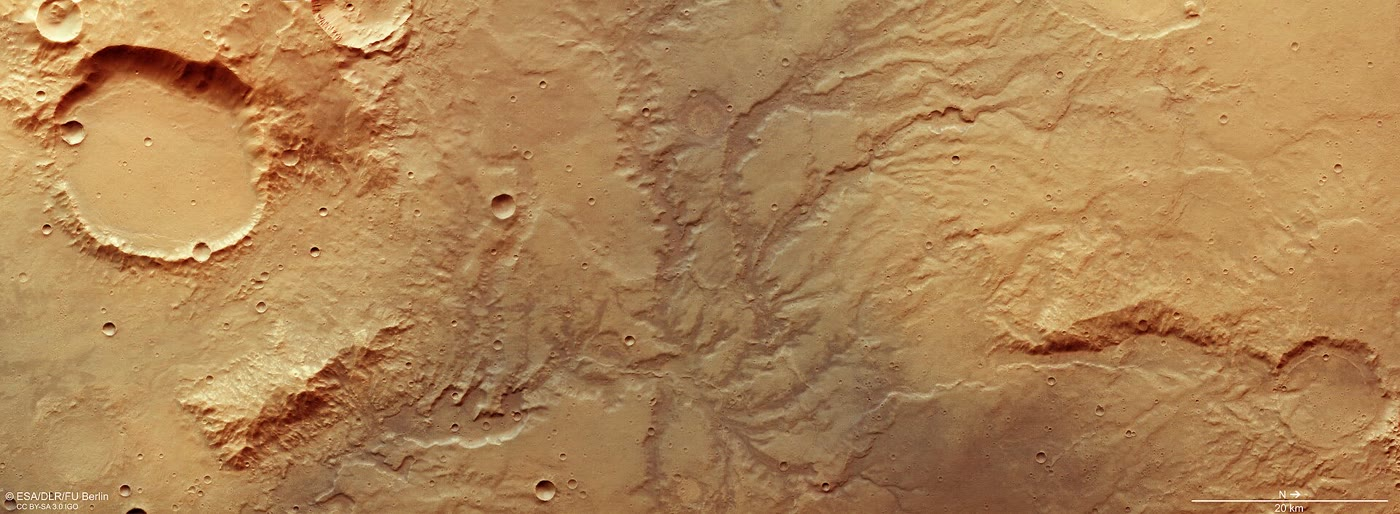
\includegraphics[width=\linewidth]{images/book5/b3-mars-valley-network.jpg}
\par\smallskip{\small A network of dried-up valleys on Mars, seen by the
camera of Mars Express at about \qty{14}{m} per pixel, near \ang{17}\,S,
\ang{66}\,E; north is to the right, and the scale bar is \qty{20}{km}.
Tributaries join downstream into larger valleys, the pattern of a
drainage network. Image ESA/DLR/FU Berlin, CC BY-SA 3.0 IGO.}\label{fig:b3:planetary-atmospheres:valleys}
\end{omfigure}
% ledger: photo:b3-mars-valley-network

The valleys and the flow channels of Mars need, by geological estimates,
a global layer of water 100 to \qty{1500}{m} deep, against 3 to
\qty{25}{m} in its ice and air today. Much of the rest went to space. The
MAVEN orbiter measured the solar wind stripping gas from Mars at about
\qty{100}{g} per second, three quarters of it down the tail
behind the planet, where the solar wind flows, and a quarter in a plume
over the poles; during the
solar storms of March 2015 the loss sped up, and it was probably much
faster when the young Sun was more active. Mars also loses hydrogen, about
\num{3e26} atoms per second on average today: kept up for four billion
years, a loss worth a global layer of water only about \qty{4}{m} deep.
% ledger: gilli25:h-loss, lasp:maven

The rate has not always been today's. The obliquity of Mars, \ang{25.2}
now, has wandered between 0 and \ang{66} over the last 250 million years,
around a mean near \ang{35}, while the Earth's varies by little more than a
degree. The motion is chaotic and cannot be traced back over billions of
years; elliptical craters made by grazing impacts, whose orientations
record the obliquity, suggest a mean between about 10 and \ang{30} over
the last 3.5 billion years or so. At high obliquity the summer pole warms,
more water vapour rises, and climate models make the loss of hydrogen
twenty times faster: over Mars's history, a layer of the order of
\qty{80}{m}.
% ledger: planet:Mars.obliq, gilli25:obliquity, holo18:obliquity, gilli25:h-loss

\section{Titan: a methane cycle}\label{sec:b3:planetary-atmospheres:titan}

Titan, a moon smaller than Mars, has a thicker atmosphere than the Earth:
a surface pressure about 60\,\% higher, at \qty{-179}{\degreeCelsius}.
The atmosphere is about 95\,\% nitrogen and 5\,\% methane, and because the
moon's gravity is weak it extends ten times higher than the Earth's, to
nearly \qty{600}{km}. Ultraviolet light splits the methane and nitrogen
high up; the fragments recombine into an orange haze of heavier
hydrocarbons that hides the surface from visible light. Below the haze,
methane plays the part of water: it condenses into clouds, rains, cuts
river channels and fills lakes and seas of methane and ethane.
% ledger: nasa:titan-surface, nasa:titan-facts

\begin{omfigure}
\centering
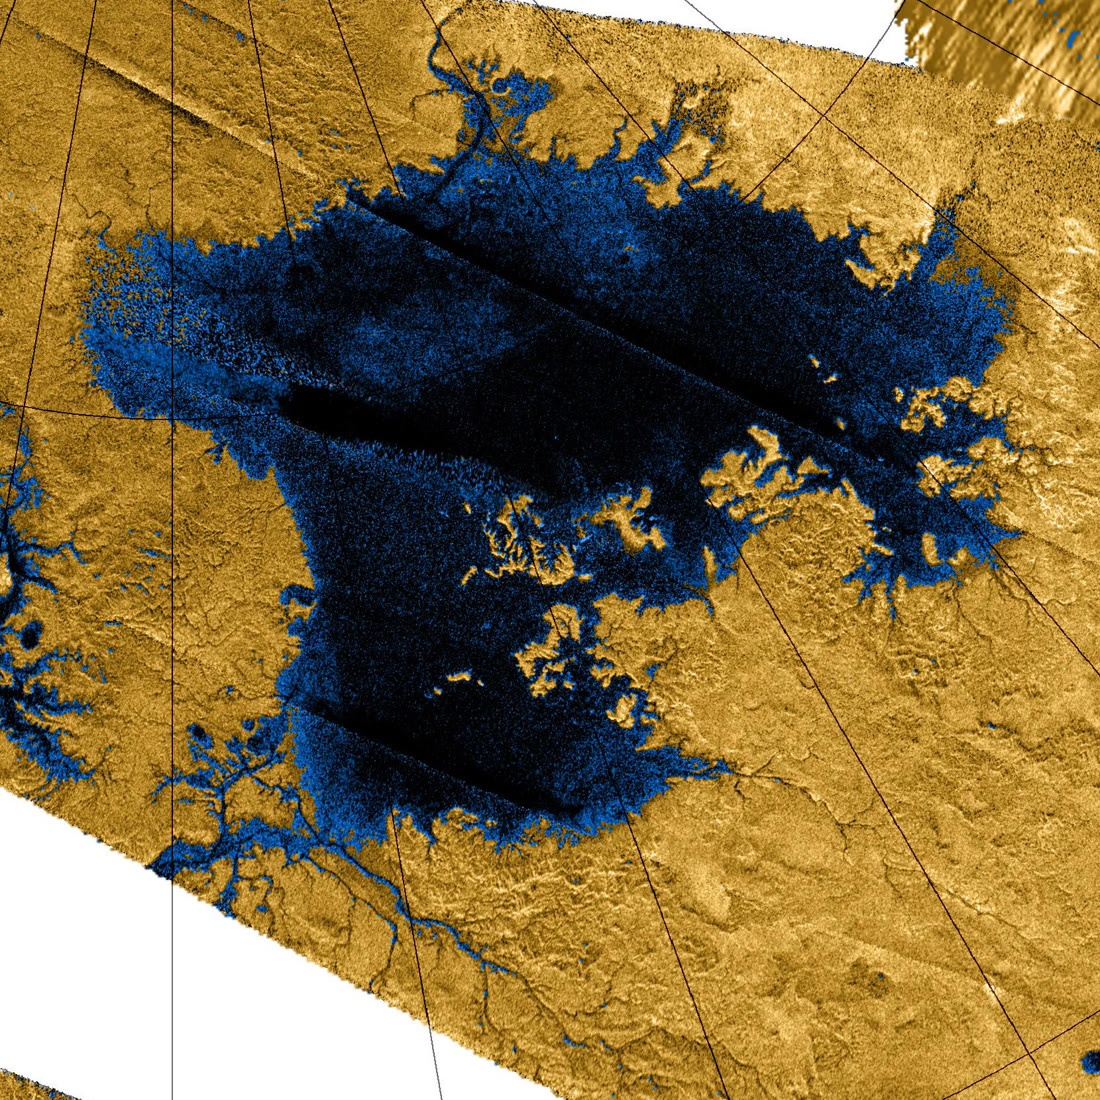
\includegraphics[width=0.5\linewidth]{images/book5/b3-ligeia-mare.jpg}
\par\smallskip{\small Ligeia Mare, a sea near Titan's north pole, in a
false-colour mosaic of Cassini radar images: features thought to be
liquid in blue and black, solid ground tinted brown, with bays, islands
and presumed tributary networks. Of about 400 lakes and seas in the mapped
north, those larger than \qty{26000}{km^2} hold 70\,\% of the area.
NASA/JPL/USGS, public domain.}\label{fig:b3:planetary-atmospheres:ligeia}
\end{omfigure}
% ledger: photo:b3-ligeia-mare

Whether a liquid can lie on a surface depends on its phase diagram and on
the pressure and temperature there. Titan's surface lies just above the
triple point of methane, \qty{90.67}{K} and \qty{0.117}{bar}, and below
its critical point: liquid methane is possible, and methane at 5\,\% of
\qty{1.6}{bar} is not far from saturation. The surface of Mars sits near
the triple point of water, the Earth's well inside its liquid field, and
Venus's above water's critical temperature, \qty{647}{K}, where no
liquid can exist at all.
% ledger: nist:methane-phase, iapws:triple-critical, nasa:titan-surface

\begin{omfigure}
\centering
\begin{tikzpicture}
\begin{axis}[width=0.8\linewidth, height=0.52\linewidth,
  xmin=60, xmax=800, ymin=1e-4, ymax=1000, ymode=log,
  xlabel={temperature (\unit{K})}, ylabel={pressure (\unit{bar})},
  tick label style={font=\scriptsize}, label style={font=\small}]
\addplot[thick, omDef] table[x=T, y=p_bar] {figdata/out/bachelor-3-habitability-water.dat};
\addplot[thick, omDef, dashed] table[x=T, y=p_bar] {figdata/out/bachelor-3-habitability-ice.dat};
\addplot[thick, orange!80!black] table[x=T, y=p_bar] {figdata/out/bachelor-3-habitability-methane.dat};
\addplot[only marks, mark=*, mark size=1.6pt, omDef] coordinates {(273.16,0.00611657) (647.096,220.64)};
\addplot[only marks, mark=*, mark size=1.6pt, orange!80!black] coordinates {(90.67,0.1169) (190.6,46.1)};
\addplot[only marks, mark=square*, mark size=2.2pt, black] table[x=T, y=p_bar] {figdata/out/bachelor-3-habitability-bodies.dat};
\node[font=\scriptsize, anchor=south] at (axis cs:737,110) {Venus};
\node[font=\scriptsize, anchor=west] at (axis cs:300,1.0) {Earth};
\node[font=\scriptsize, anchor=north] at (axis cs:214,0.0045) {Mars};
\node[font=\scriptsize, anchor=south] at (axis cs:94,2.2) {Titan};
\node[font=\scriptsize, omDef, anchor=west] at (axis cs:420,3) {water: liquid above, vapour below};
\node[font=\scriptsize, omDef, anchor=north west] at (axis cs:205,0.0012) {ice};
\node[font=\scriptsize, orange!80!black, anchor=west] at (axis cs:196,46) {methane};
\node[font=\scriptsize, omDef, anchor=south east] at (axis cs:640,230) {critical point};
\end{axis}
\end{tikzpicture}
\par\smallskip{\small The boundaries between vapour and condensed water
(blue: liquid--vapour, from the triple point to the critical point;
dashed: ice--vapour) and between liquid methane and its vapour (orange),
with the mean surface states of Venus, the Earth, Mars and Titan
(squares). A liquid can lie on a surface whose pressure is above the
curve of that liquid, between its triple and critical
temperatures.}\label{fig:b3:planetary-atmospheres:phases}
\end{omfigure}
% ledger: iapws:vapour-pressure, iapws4:sublimation, iapws:triple-critical, nist:methane-phase, nasa:venus-atm, planet:Earth.Tmean, planet:Earth.psurf, nasa:mars-atm, nasa:titan-surface

Titan keeps its nitrogen easily: at its \omterm{def:b3:planetary-atmospheres:exobase}{exobase} $\lambda = 41$ for
nitrogen. Its hydrogen, at $\lambda$ near 1.5, leaves almost freely, and
the escape of molecular hydrogen is set lower down by the limiting flux
through the \omterm{def:b3:planetary-atmospheres:hydrodynamic}{homopause}, as on the Earth. The heavy compounds made from the
broken methane settle to the surface, where they make the sand of vast
fields of dunes.
% ledger: gronoff:jeans-table, gronoff:diffusion, nasa:titan-surface

\section{Planetary habitability}\label{sec:b3:planetary-atmospheres:habitability}

The habitable zone of the school books is the range of distances from a
star at which a planet like the Earth can keep liquid water at its
surface. Its edges are the limits met in this chapter.

\begin{definition}[Planetary habitability]\label{def:b3:planetary-atmospheres:habitability}
The \emph{planetary habitability}\index{planetary habitability} of a
planet is its capacity to keep liquid water at its surface over
geological times: it receives a stellar flux within the limits of the
habitable zone, it holds on to its atmosphere and its water against
escape, and a long-term carbon cycle regulates its climate.
\end{definition}

The inner edge of the habitable zone is the moist or the \omterm{def:b3:planetary-atmospheres:runaway}{runaway
greenhouse}: an Earth-like planet around the Sun turns moist at
\qty{0.99}{au} and runs away at \qty{0.97}{au}. The outer edge is the
\emph{maximum greenhouse}: adding carbon dioxide warms a planet only until
the extra gas scatters back more sunlight than its greenhouse effect
gains; around the Sun this happens at
\qty{1.70}{au}, under some \qty{8}{bar} of carbon dioxide. Those are
conservative edges, computed without clouds. Two empirical ones are wider:
Venus seems to have had no surface water for at least a billion years,
when it received 1.76 times the Earth's present sunlight (\qty{0.75}{au});
Mars had flowing water when it received 0.32 times that sunlight, if its
valleys are 3.8 billion years old (\qty{1.77}{au}). Around cooler stars the same limits come
at lower fluxes, because their redder light is scattered less and absorbed
more by water and carbon dioxide.
% ledger: kopparapu13:runaway, kopparapu13:outer, kopparapu13:hz-fit

\begin{omfigure}
\centering
\begin{tikzpicture}
\begin{axis}[width=0.8\linewidth, height=0.5\linewidth,
  xmin=0, xmax=2.1, ymin=2600, ymax=7200, x dir=reverse,
  xlabel={stellar flux received / Earth's today},
  ylabel={stellar temperature (\unit{K})},
  tick label style={font=\scriptsize}, label style={font=\small},
  legend style={font=\scriptsize, at={(0.5,-0.24)}, anchor=north, legend columns=2, draw=none}]
\addplot[name path=mg, thick, omDef] table[x=mg, y=Teff] {figdata/out/bachelor-3-habitability-hz.dat};
\addlegendentry{moist greenhouse}
\addplot[name path=maxg, thick, red!70!black] table[x=maxg, y=Teff] {figdata/out/bachelor-3-habitability-hz.dat};
\addlegendentry{maximum greenhouse}
\addplot[thin, omDef, dashed] table[x=rg, y=Teff] {figdata/out/bachelor-3-habitability-hz.dat};
\addlegendentry{runaway greenhouse}
\addplot[thin, black!60, densely dotted] table[x=rv, y=Teff] {figdata/out/bachelor-3-habitability-hz.dat};
\addlegendentry{recent Venus, early Mars}
\addplot[thin, black!60, densely dotted, forget plot] table[x=em, y=Teff] {figdata/out/bachelor-3-habitability-hz.dat};
\addplot[green!30, opacity=0.5, forget plot] fill between[of=mg and maxg];
\addplot[only marks, mark=*, mark size=2pt, black, forget plot] coordinates {(1.911,5780) (1.0,5780) (0.431,5780)};
\node[font=\scriptsize, anchor=south] at (axis cs:1.911,5800) {Venus};
\node[font=\scriptsize, anchor=west, xshift=2pt] at (axis cs:1.0,5780) {Earth};
\node[font=\scriptsize, anchor=east, xshift=-2pt] at (axis cs:0.431,5780) {Mars};
\end{axis}
\end{tikzpicture}
\par\smallskip{\small The habitable zone of an Earth-like planet, as the
stellar flux it receives against the temperature of its star (shaded:
between the \omterm{def:b3:planetary-atmospheres:runaway}{moist greenhouse} and the maximum greenhouse). Dotted: the
empirical limits drawn from recent Venus and early Mars. The fits are
those of a cloud-free climate model, valid from 2600 to
\qty{7200}{K}.}\label{fig:b3:planetary-atmospheres:hz}
\end{omfigure}
% ledger: kopparapu13:hz-fit, nasa:venus, nasa:mars

Distance is not enough. A planet must hold on to its atmosphere: a small
or hot one, whose \omterm{def:b3:planetary-atmospheres:jeans-escape}{escape parameter} is low, loses its hydrogen and with it
its water, and a planet in a \omterm{def:b3:planetary-atmospheres:runaway}{moist greenhouse} dries out from the top. It
must also keep its climate stable over billions of years while its star
brightens: on the Earth, the silicate-weathering thermostat of the
long-term carbon cycle draws carbon dioxide down when the climate warms
and lets it build up when it cools. On Venus, without plate tectonics,
outgassed carbon dioxide has had no way back into the rocks and has
accumulated in the air; it now holds about as much carbon dioxide as the
Earth has locked in carbonate rocks. Whether a magnetic field protects an
atmosphere is debated: it shields the upper atmosphere from the solar
wind, but it also opens other paths of escape, such as the outflow of ions
near the poles, and the habitability of a planet cannot be read from its
place in the habitable zone alone.
% ledger: arney18:venus-loss, gronoff21:magnetic, gronoff:nonthermal

\section{Exercises}

\begin{exercise}[$\star$]\label{exo:b3:planetary-atmospheres:1}
Compute the scale height $H = RT/Mg$ near the surface of Venus
(\qty{737}{K}, carbon dioxide of molar mass \qty{44.01}{g.mol^{-1}},
$g = \qty{8.87}{m.s^{-2}}$), the Earth (\qty{288}{K},
\qty{28.97}{g.mol^{-1}}, \qty{9.80}{m.s^{-2}}), Mars (\qty{214}{K},
\qty{43.34}{g.mol^{-1}}, \qty{3.71}{m.s^{-2}}) and Titan (\qty{94}{K},
\qty{28.0}{g.mol^{-1}}, \qty{1.35}{m.s^{-2}}). Which atmosphere is the
most extended, and why?
\end{exercise}

\begin{exercise}[$\star$]\label{exo:b3:planetary-atmospheres:2}
The Earth's \omterm{def:b3:planetary-atmospheres:exobase}{exobase} lies at \qty{500}{km} (radius \qty{6878}{km}); its
temperature varies from 800 to \qty{1600}{K} over the solar cycle. Take
the mass of the Earth as \qty{5.97e24}{kg}. Compute the \omterm{def:b3:planetary-atmospheres:jeans-escape}{escape parameter}
of hydrogen atoms at both temperatures, and the escaping fraction
$(1 + \lambda)e^{-\lambda}$. By what factor does the solar cycle change it?
\end{exercise}

\begin{exercise}[$\star$]\label{exo:b3:planetary-atmospheres:3}
Around the Sun, an Earth-like planet turns moist at the flux $S_\mathrm{eff}
= 1.014$, runs away at 1.0512 and reaches the maximum greenhouse at 0.3438
(fluxes relative to the Earth's). (a)~Compute the three distances, in
astronomical units. (b)~Venus and Mars receive 1.91 and 0.43 times the
Earth's sunlight. Place them.
\end{exercise}

\begin{exercise}[$\star$]\label{exo:b3:planetary-atmospheres:4}
The vapour pressure of liquid methane is $\log_{10}(p/\unit{bar}) = 3.9895 -
443.028/(T/\unit{K} - 0.49)$. (a)~Compute it at the surface of Titan,
\qty{94.15}{K}. (b)~Methane makes 5\,\% of Titan's air at \qty{1.6}{bar}.
Compute its partial pressure and its relative humidity. (c)~What does
the result suggest about evaporation from Titan's seas?
\end{exercise}

\begin{exercise}[$\star\star$]\label{exo:b3:planetary-atmospheres:5}
At the Earth's \omterm{def:b3:planetary-atmospheres:exobase}{exobase} (\qty{1000}{K}, $\lambda = 7.02$ for hydrogen),
compute the \omterm{def:b3:planetary-atmospheres:jeans-escape}{escape parameter} of deuterium, its thermal speed relative to
hydrogen's and the ratio of the Jeans fluxes per atom, D to H. Is \omterm{def:b3:planetary-atmospheres:jeans-escape}{Jeans
escape} a strong isotopic filter?
\end{exercise}

\begin{exercise}[$\star\star$]\label{exo:b3:planetary-atmospheres:6}
The ratio D/H of the water of Venus is \num{0.016}; that of ocean water on
the Earth is \num{1.5575e-4}. (a)~Compute the enrichment. (b)~With no
escape of deuterium at all, what is the smallest past inventory of water
of Venus, given \qty{6e15}{kg} today? What depth would it make spread over
the planet's \qty{4.60e14}{m^2}? (c)~What shrinking of the reservoir would
\omterm{def:b3:planetary-atmospheres:hydrodynamic}{diffusion-limited escape}, with $\alpha = 0.8$, require? Conclude.
\end{exercise}

\begin{exercise}[$\star\star$]\label{exo:b3:planetary-atmospheres:7}
Mars, of radius \qty{3389.5}{km}, loses about \num{3e26} hydrogen atoms
per second. (a)~If each pair of atoms came from a molecule of water, what
global layer of water does the loss remove in four billion years?
(b)~Same question at \num{6e27} atoms per second, the rate of a high
obliquity. (c)~Compare with the 100 to \qty{1500}{m} the valleys and
channels need.
\end{exercise}

\begin{exercise}[$\star\star$]\label{exo:b3:planetary-atmospheres:8}
(a)~Compute the mass of the atmosphere of Mars from its mean surface
pressure, \qty{636}{Pa}, its gravity, \qty{3.71}{m.s^{-2}}, and its
radius. (b)~The solar wind strips about \qty{100}{g} of gas per second.
What mass does that remove in four billion years, and in how long would
it remove the present atmosphere? (c)~Why is that an underestimate of the
past loss?
\end{exercise}

\begin{exercise}[$\star\star$]\label{exo:b3:planetary-atmospheres:9}
An Earth-like planet with a cloud-free steam atmosphere reflects 19.3\,\%
of the sunlight it receives; its infrared output cannot exceed
\qty{291}{W.m^{-2}}. (a)~Above what flux of sunlight, in watts per square
metre and relative to the Earth's \qty{1361}{W.m^{-2}}, does it run away?
(b)~Compare with Venus today, \qty{2601}{W.m^{-2}}, and with a young Venus
under a Sun at 70\,\% of its present luminosity. (c)~Why is the
conclusion for the young Venus not final?
\end{exercise}

\begin{exercise}[$\star\star\star$]\label{exo:b3:planetary-atmospheres:10}
A model thermosphere of atomic oxygen is isothermal at \qty{1000}{K}, with
$n = \qty{1e16}{m^{-3}}$ at \qty{200}{km}; take $g =
\qty{9.21}{m.s^{-2}}$ at that height and a collision cross-section
$\sigma_c = \qty{3e-19}{m^2}$. (a)~Compute the scale height of the oxygen.
(b)~Compute the density at the \omterm{def:b3:planetary-atmospheres:exobase}{exobase} and the height of the \omterm{def:b3:planetary-atmospheres:exobase}{exobase}.
(c)~Gravity decreases with height. Does that move the \omterm{def:b3:planetary-atmospheres:exobase}{exobase} up or
down?
\end{exercise}

\begin{exercise}[$\star\star\star$]\label{exo:b3:planetary-atmospheres:11}
(a)~Suppose the Earth's stratosphere turned moist, with a mixing ratio of
water vapour of \num{3e-3} (counted as $\ce{H2}$). With the diffusion
limit $\num{3.0e13}\,f$ molecules of $\ce{H2}$ per square centimetre and
per second, at \qty{200}{K}, compute the loss of hydrogen of the whole
Earth (radius \qty{6371}{km}). (b)~How long would an ocean,
\qty{1.4e24}{g} of water, last? Compare with the age of the Earth.
\end{exercise}

\begin{exercise}[$\star\star\star$]\label{exo:b3:planetary-atmospheres:12}
In a pure-steam upper atmosphere absorbing as a grey gas with $\kappa =
\qty{0.005}{m^2.kg^{-1}}$, on a planet with $g = \qty{9.81}{m.s^{-2}}$
and $D = 1.66$: (a)~compute the pressure $p_1$ of the radiating level;
(b)~with $p_\mathrm{sat}(T) = \qty{611.657}{Pa}\,\exp[(L/R_v)(1/T_t -
1/T)]$, $L = \qty{2.5e6}{J.kg^{-1}}$, $R_v = \qty{461.5}{J.kg^{-1}.K^{-1}}$,
$T_t = \qty{273.16}{K}$, compute its temperature and the radiation limit.
(c)~The line-by-line limit is \qty{291}{W.m^{-2}}. Should the effective
$\kappa$ of real water vapour be larger or smaller?
\end{exercise}

\section{Problem: Will Kepos Keep Its Water?}

\begin{problem}[{Weekend problem --- escape and habitability of an invented
ocean planet}]
\label{pb:b3:planetary-atmospheres:1}
Kepos is an invented planet of mass \qty{5.2e24}{kg} and radius
\qty{6200}{km}, with oceans and an atmosphere of nitrogen and carbon
dioxide. It orbits at \qty{0.60}{au} a star of luminosity 0.30 times the
Sun's and effective temperature \qty{4800}{K}. Its \omterm{def:b3:planetary-atmospheres:exobase}{exobase} lies
\qty{500}{km} above the surface, at \qty{1400}{K}, with
\qty{2e11}{m^{-3}} hydrogen atoms; its \omterm{def:b3:planetary-atmospheres:hydrodynamic}{homopause} is at \qty{200}{K},
where carbon dioxide dominates and where hydrogen in all its forms makes a
mixing ratio $f = \num{1e-3}$, counted as $\ce{H2}$. An Earth ocean is
\qty{1.4e24}{g} of water.

\medskip\noindent\textbf{Part I --- The exobase.}
\begin{enumerate}
\item Compute the surface gravity and the mean density of Kepos.
\item Compute the escape velocity at the \omterm{def:b3:planetary-atmospheres:exobase}{exobase}.
\item Compute the thermal speed $u = \sqrt{2kT/m}$ of hydrogen, helium and
  oxygen atoms at the \omterm{def:b3:planetary-atmospheres:exobase}{exobase}.
\item Compute their \omterm{def:b3:planetary-atmospheres:jeans-escape}{escape parameters}.
\item Which of them can escape by \omterm{def:b3:planetary-atmospheres:jeans-escape}{Jeans escape} at a significant rate?
  Is any close to the hydrodynamic regime?
\item During an active youth of its star the \omterm{def:b3:planetary-atmospheres:exobase}{exobase} of Kepos may have
  reached \qty{3000}{K}. What was then the \omterm{def:b3:planetary-atmospheres:jeans-escape}{escape parameter} of hydrogen,
  and what does it suggest?
\end{enumerate}

\medskip\noindent\textbf{Part II --- Jeans escape of hydrogen.}
\begin{enumerate}[resume]
\item Compute the escaping fraction $(1 + \lambda)e^{-\lambda}$ for
  hydrogen.
\item Compute the Jeans flux of hydrogen, per square metre and per second.
\item Compute the number of hydrogen atoms that leave the whole \omterm{def:b3:planetary-atmospheres:exobase}{exobase}
  per second.
\item How many hydrogen atoms does an Earth ocean hold?
\item At this rate, how long would Kepos take to lose them?
\item Compute the \omterm{def:b3:planetary-atmospheres:jeans-escape}{escape parameter} of deuterium and its escape efficiency
  relative to hydrogen, per atom.
\end{enumerate}

\medskip\noindent\textbf{Part III --- The diffusion limit.}
\begin{enumerate}[resume]
\item Compute the scale height of carbon dioxide at the \omterm{def:b3:planetary-atmospheres:hydrodynamic}{homopause}.
\item The binary diffusion parameter of hydrogen in carbon dioxide is
  $b = \qty{1.2e19}{cm^{-1}.s^{-1}}$ at \qty{200}{K}. Compute the
  diffusion-limited flux of $\ce{H2}$, per square metre and per second.
\item Check it against the Earth's limit, $\num{3.0e13}\,f$ molecules per
  square centimetre and per second, scaled by gravity.
\item Compute the number of hydrogen atoms that the diffusion limit can
  supply to the upper atmosphere of the whole planet per second (take the
  area of the surface).
\item Compare with question~9. Which process limits the escape, and what
  happens to the hydrogen of the thermosphere?
\item What density of hydrogen at the \omterm{def:b3:planetary-atmospheres:exobase}{exobase} would let \omterm{def:b3:planetary-atmospheres:jeans-escape}{Jeans escape} carry
  the whole supply?
\item How long would Kepos take to lose an Earth ocean of hydrogen at the
  diffusion limit?
\end{enumerate}

\medskip\noindent\textbf{Part IV --- Is Kepos in the habitable zone?}
\begin{enumerate}[resume]
\item Compute the stellar flux Kepos receives, relative to the Earth's.
\item For a star of \qty{4800}{K} the \omterm{def:b3:planetary-atmospheres:runaway}{moist greenhouse} limit is at
  $S_\mathrm{eff} = 0.939$ and the maximum greenhouse at 0.290. Compute the
  edges of the habitable zone, in astronomical units, and place Kepos.
\item By what factor must the star brighten before Kepos reaches the inner
  edge?
\item With an albedo of 0.3, compute the sunlight Kepos absorbs per square
  metre, and its equilibrium temperature. Compare with the \omterm{def:b3:planetary-atmospheres:runaway}{runaway
  greenhouse limit}.
\item If a warmer climate made the stratosphere of Kepos moist, with
  $f = \num{3e-3}$, how long would an Earth ocean last?
\item Give the time for Kepos to lose an Earth ocean of hydrogen by
  \omterm{def:b3:planetary-atmospheres:hydrodynamic}{diffusion-limited escape} with $f = \num{1e-3}$, in billions of years, to
  two significant figures.
\end{enumerate}
\end{problem}
% ledger: zahnle19:diffusion, kopparapu13:hz-fit, kopparapu13:runaway, gronoff:jeans, const:G, const:kB, const:NA
